% Options for packages loaded elsewhere
\PassOptionsToPackage{unicode}{hyperref}
\PassOptionsToPackage{hyphens}{url}
\documentclass[
]{article}
\usepackage{xcolor}
\usepackage{amsmath,amssymb}
\setcounter{secnumdepth}{-\maxdimen} % remove section numbering
\usepackage{iftex}
\ifPDFTeX
  \usepackage[T1]{fontenc}
  \usepackage[utf8]{inputenc}
  \usepackage{textcomp} % provide euro and other symbols
\else % if luatex or xetex
  \usepackage{unicode-math} % this also loads fontspec
  \defaultfontfeatures{Scale=MatchLowercase}
  \defaultfontfeatures[\rmfamily]{Ligatures=TeX,Scale=1}
\fi
\usepackage{lmodern}
\ifPDFTeX\else
  % xetex/luatex font selection
\fi
% Use upquote if available, for straight quotes in verbatim environments
\IfFileExists{upquote.sty}{\usepackage{upquote}}{}
\IfFileExists{microtype.sty}{% use microtype if available
  \usepackage[]{microtype}
  \UseMicrotypeSet[protrusion]{basicmath} % disable protrusion for tt fonts
}{}
\makeatletter
\@ifundefined{KOMAClassName}{% if non-KOMA class
  \IfFileExists{parskip.sty}{%
    \usepackage{parskip}
  }{% else
    \setlength{\parindent}{0pt}
    \setlength{\parskip}{6pt plus 2pt minus 1pt}}
}{% if KOMA class
  \KOMAoptions{parskip=half}}
\makeatother
\usepackage{graphicx}
\makeatletter
\newsavebox\pandoc@box
\newcommand*\pandocbounded[1]{% scales image to fit in text height/width
  \sbox\pandoc@box{#1}%
  \Gscale@div\@tempa{\textheight}{\dimexpr\ht\pandoc@box+\dp\pandoc@box\relax}%
  \Gscale@div\@tempb{\linewidth}{\wd\pandoc@box}%
  \ifdim\@tempb\p@<\@tempa\p@\let\@tempa\@tempb\fi% select the smaller of both
  \ifdim\@tempa\p@<\p@\scalebox{\@tempa}{\usebox\pandoc@box}%
  \else\usebox{\pandoc@box}%
  \fi%
}
% Set default figure placement to htbp
\def\fps@figure{htbp}
\makeatother
\setlength{\emergencystretch}{3em} % prevent overfull lines
\providecommand{\tightlist}{%
  \setlength{\itemsep}{0pt}\setlength{\parskip}{0pt}}
\usepackage[]{biblatex}
\usepackage{bookmark}
\IfFileExists{xurl.sty}{\usepackage{xurl}}{} % add URL line breaks if available
\urlstyle{same}
\hypersetup{
  hidelinks,
  pdfcreator={LaTeX via pandoc}}

\author{}
\date{}

\begin{document}

\section{Findings}\label{findings}

I focus on a string of episodes where Jane, a promising trench assistant
working at an archaeological project, learned to identify,
differentiate, and document parts of a stratigraphic sequence. I
illustrate how the constitution of the archaeological record, and the
internalization of archaeological knowledge, occurred as part of project
frameworks and collaborative relations that were structured by projects'
divisions of labour.

\subsection{Learning to see like an
archaeologist}\label{learning-to-see-like-an-archaeologist}

As illustrated in \textcite{fig-context-change}, Jane explained to me
how she identified and differentiated a new context that she was
beginning to expose in her trench, using a series of gestures paired
with speech to help convey what she meant to
say.\textsuperscript{\hyperref[sec-A1]{A1}} Jane kicked the boulders as
she referred to them, literally pointed out relations to previous
experiences that she deemed relevant, and described certain aspects of
the soil by miming the ways that she would interact with them. She
referred to common nomenclature outlined in the project's standard
recording schema and referenced by more experienced personnel, and drew
from her experiences working in other trenches that others may have
shared. More generally, she described the context change only in terms
of her interactions with it, and as framed by her particular role in the
project.

\begin{figure}
\centering
\pandocbounded{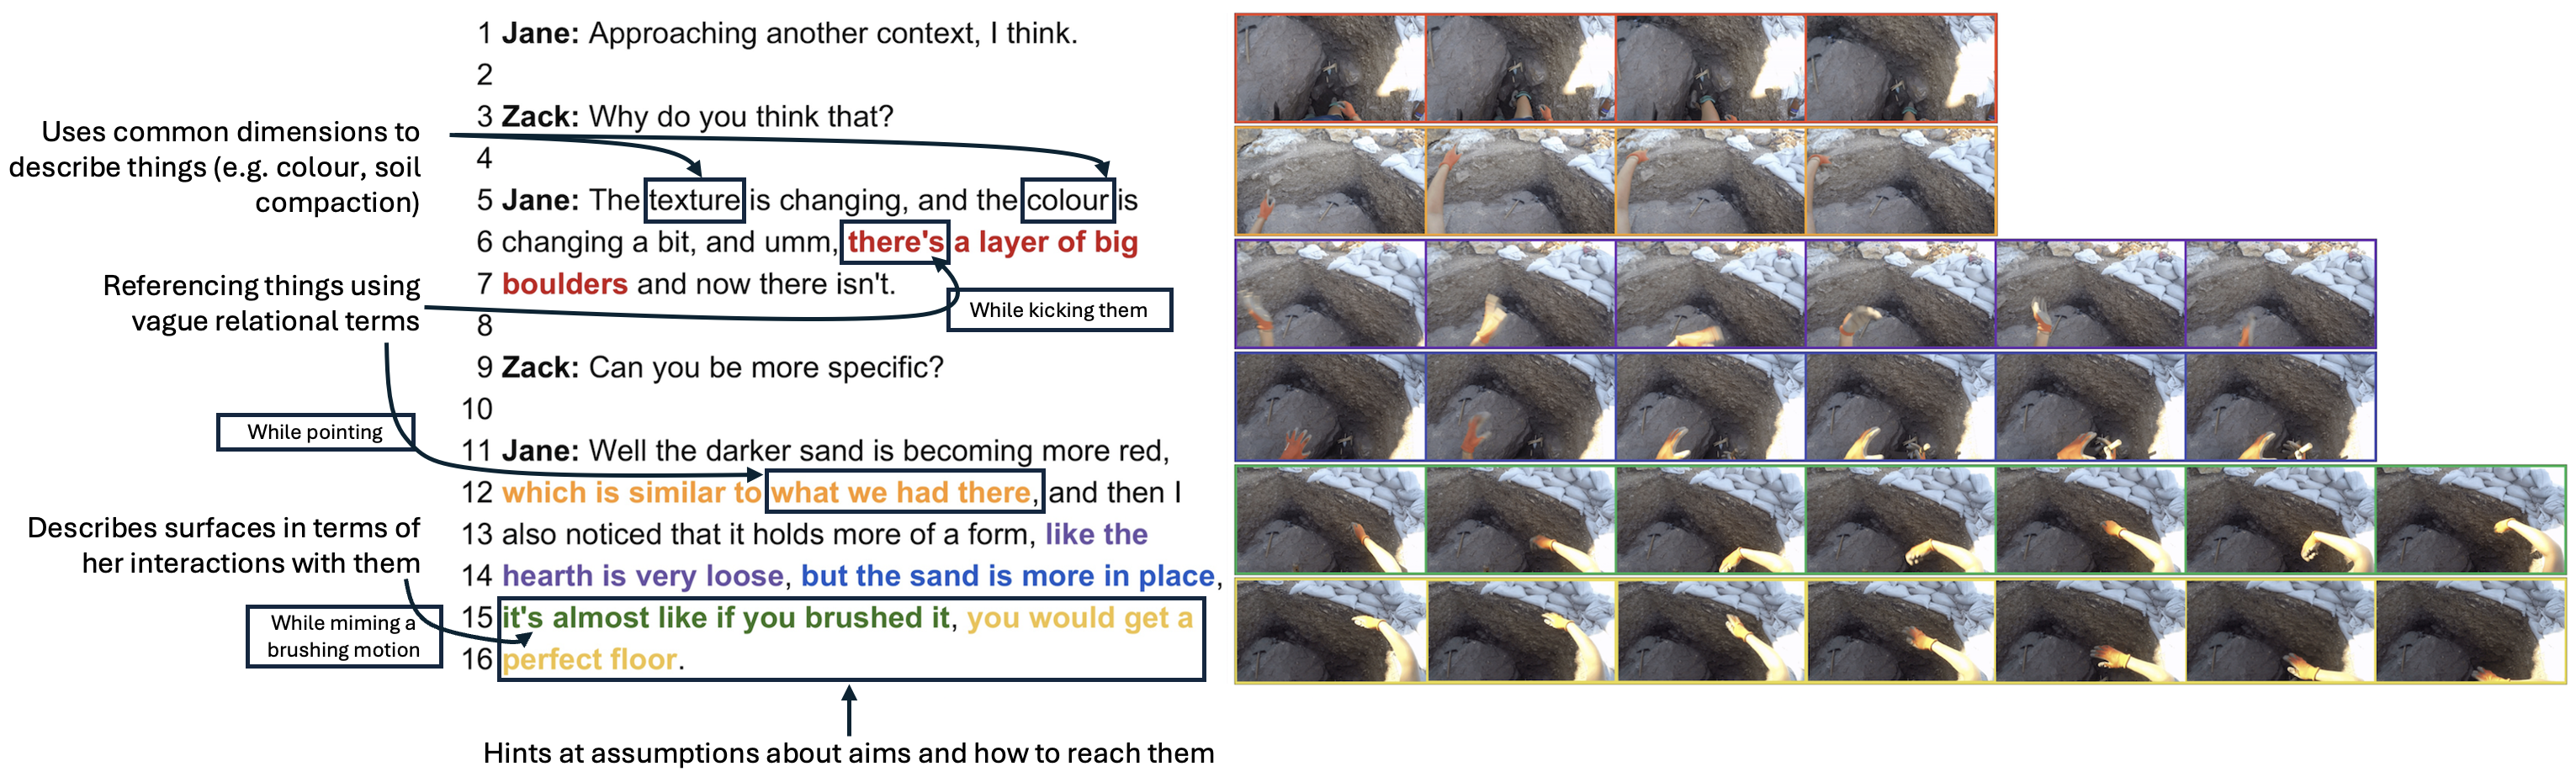
\includegraphics[keepaspectratio]{figures/context-change-annotated.png}}
\caption{Discussion of a potential context change using gestures and
speech.}\label{fig-context-change}
\end{figure}

Afterward, and as illustrated in
\textcite{fig-context-change-discussion}, Jane consulted with Basil, who
supervised work in this trench, and who is also the project director,
regarding her interpretation of the soil in
it.\textsuperscript{\hyperref[sec-A2]{A2}} Jane explained what she saw,
in terms of her encounters with the entities she identified, while
punctuating her observations with physical gestures that underscored
certainty that the entities she was observing actually exist. Basil came
to take a closer look and translated Jane's situated experiences into
more nominal and normalized terms, that distance the observer from the
observed entities. Basil then identified a series of actions that Jane
must implement, and summarized the situation by joining what was
observed with what was to be done about it, in effect rendering a
conclusive and well-reasoned decision. All the while, Jane confirmed her
understanding of Basil's corrections and of his specific instructions.

\begin{figure}
\centering
\pandocbounded{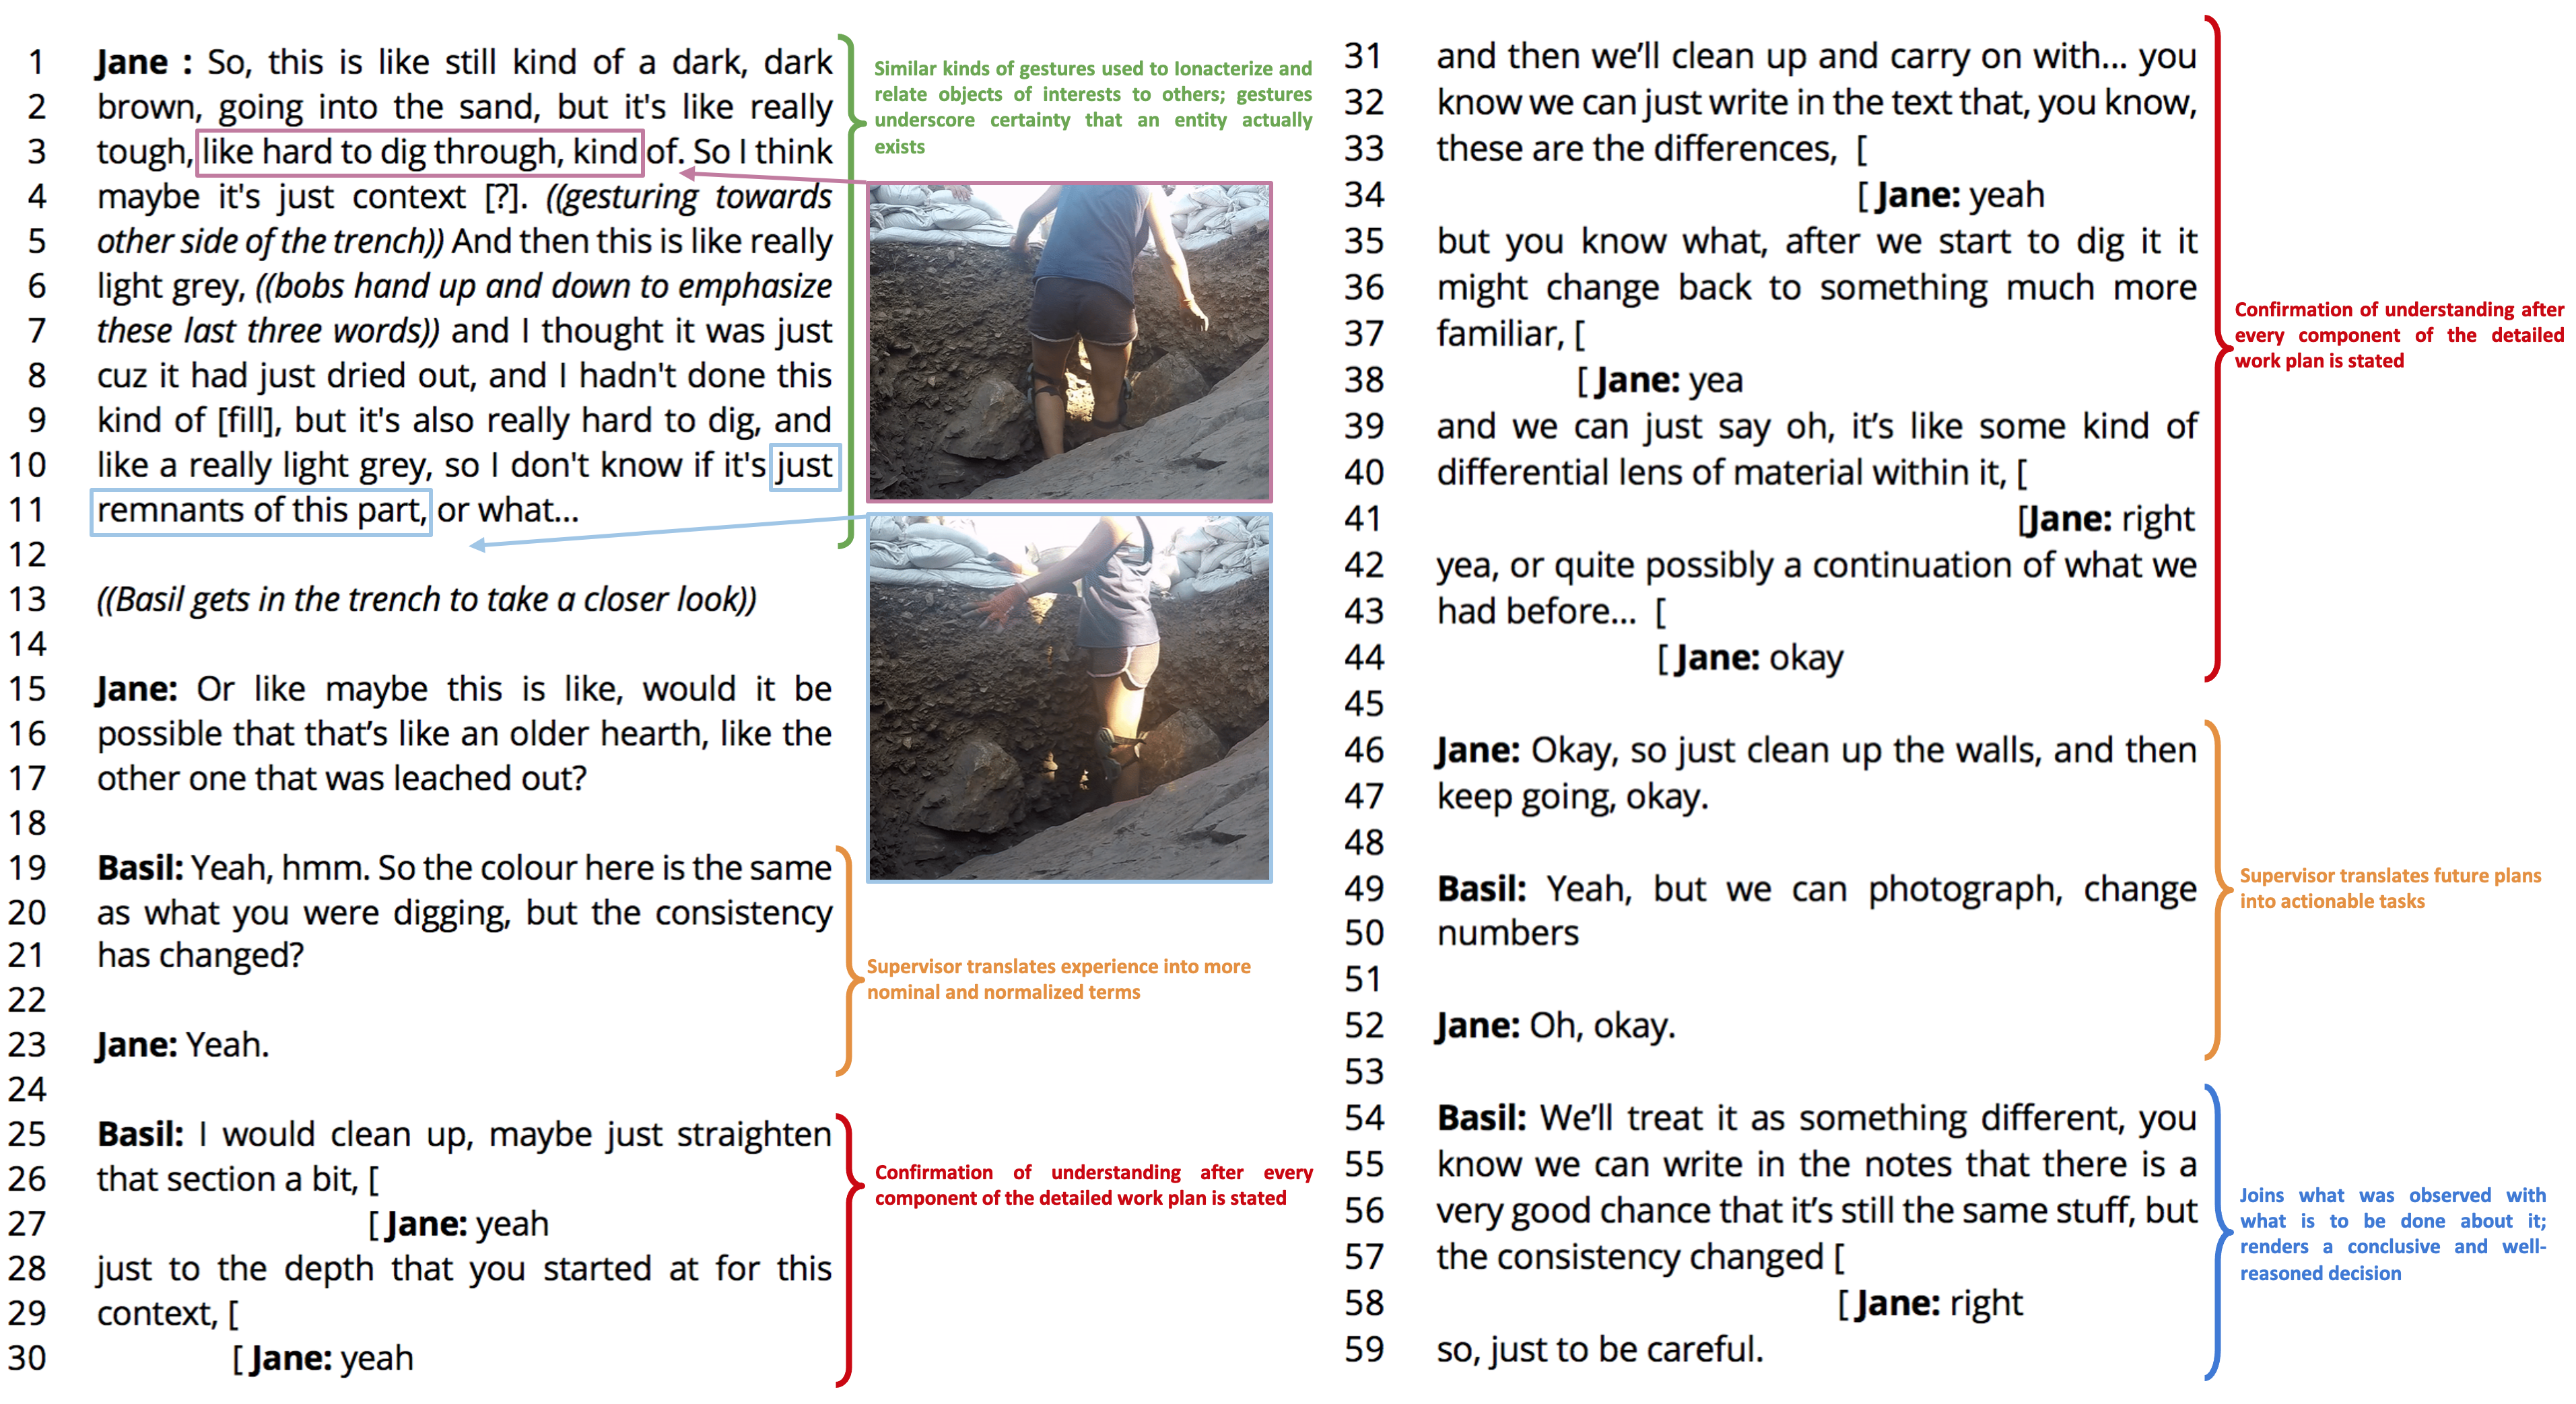
\includegraphics[keepaspectratio]{figures/context-change-discussion.png}}
\caption{Explanation of a potential context change using gestures and
speech.}\label{fig-context-change-discussion}
\end{figure}

When Jane explained her interpretation of the soil to her supervisor, he
then responded with tentative agreement, paired with his own gestures
and intonations that subtly communicated his agreement or disagreement.
The conversation between Jane and Basil therefore served as a means of
calibrating their experiences, using an independent framework as a
common reference point. In effect, Basil attempted to align Jane's
emerging perspective with a professional outlook on the sediment's
character.

As Jane stated in a subsequent interview \autocite{fig-training-eye},
she initially found it difficult to ``train her eye to see what they're
seeing'', and ``they'' seems to refer to more senior and specialized
archaeologists, including her supervisor the director, and Alfred, one
of the field directors.\textsuperscript{\hyperref[sec-A3]{A3}} By
talking through their observations in an explicit manner and in the
presence of the entities of mutual concern, while also referencing
concrete characteristics of the soil, Basil trained Jane to see things
in a way that corresponds to a formal model of how to differentiate
soil, and contexts as an natural extension of that ability. This made
him more confident in Jane's ability to recognize and report her
experiences, upon which Basil depends; as he recalled in a separate
interview, Basil came to trust Jane ``to either make her own decisions
or be responsible enough to ask other people to help her make decisions
for those moments when I'm not
there.''\textsuperscript{\hyperref[sec-A4]{A4}} This was because Jane
became capable of deciding for herself when and how to distinguish
between sediments, having internalized a conceptual framework that
affords professional legitimacy to her observational techniques.

\begin{figure}
\centering
\pandocbounded{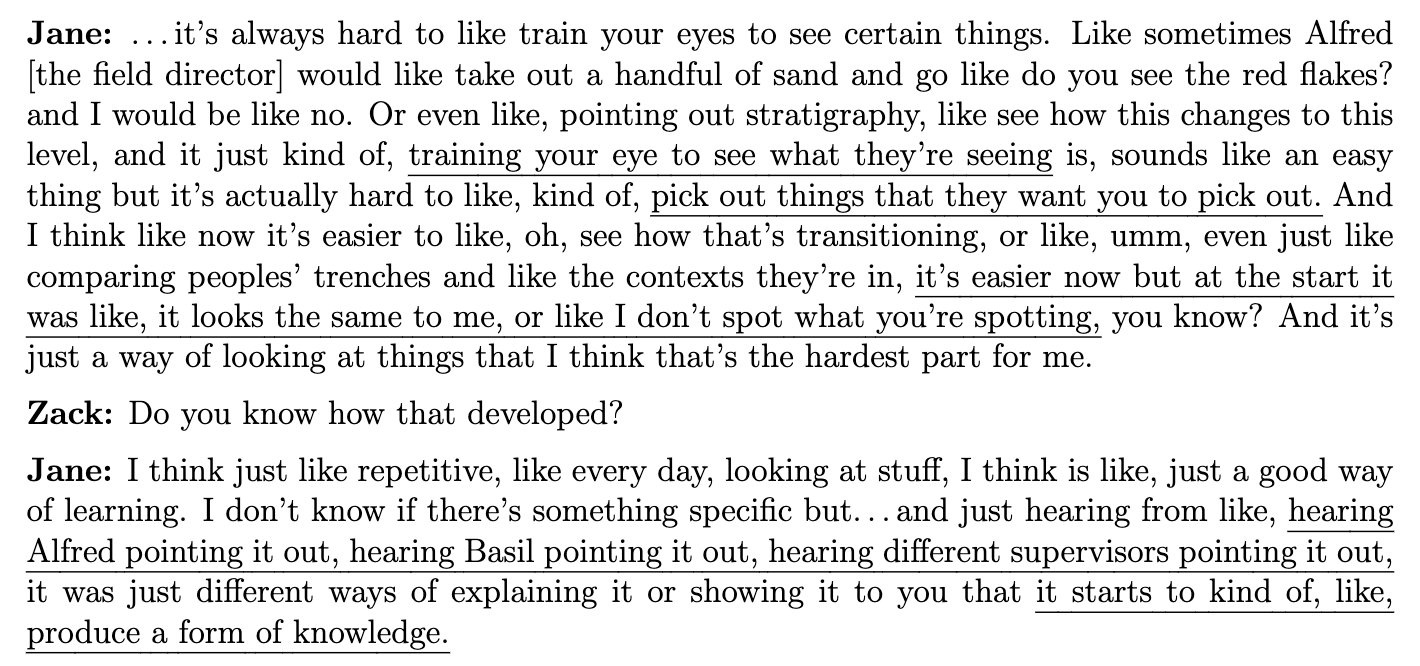
\includegraphics[keepaspectratio]{figures/training-eye.png}}
\caption{Jane describes how she learned to recognize differences in the
soil. Underlined text refer to especially significant eliciations
elucidated above.}\label{fig-training-eye}
\end{figure}

Jane's internalization of the broader conceptual framework accomplished
a few important things: (a) it aligned her own vision as part of a
collectively-held way of perceiving the world, which is led by
authoritative actors who exhibit greater creative control; (b) it
rendered her own unique experiences as generic contributions to the
project's information commons, which has the effect of reducing her
individual agency while also drawing her into a class of related agents
serving similar data collection functions, e.g.~student labourers; and
(c) it re-framed her embodied and sensory experience as a matter of
information modelling, which occurs outside material space and
circumstantial moments in time. By clarifying relatively ambiguous
perceptions through a carefully calibrated prism, the project may obtain
sharper and more well-defined outlines of the things they target for
observation, while correcting for and making it easier to dismiss the
particular embodied experiences that are collectively focused through
the aggregative lens.

\subsection{Shedding the body}\label{shedding-the-body}

I should note that Jane did not actually object to the reduction of her
situated experience in favour of more generic forms of representing the
stratigraphy. In fact, this conformed with a pattern of behaviour ---
which was enacted by all the fieldworkers I spoke with --- whereby they
tried not to think too much while excavating, opting instead to operate
in the moment, face the task at hand, and deal with what is immediately
in front of them, literally and
figuratively.\textsuperscript{\hyperref[sec-A5]{A5},\hyperref[sec-A6]{A6}}
This conformed with the expectation that the things an excavator
uncovers will gradually reveal themselves, and that she should passively
follow what is occurring in the earth before her.

To help accomplish this, fieldworkers modified the environments in which
they worked. For instance, some fieldworkers focused better while
listening to music or while blocking out social
distractions.\textsuperscript{\hyperref[sec-A7]{A7},\hyperref[sec-A8]{A8}}
Ben, who worked as an assistant in a separate trench, said that
listening to music helped him avoid being too
self-aware\textsuperscript{\hyperref[sec-A7]{A7}} while Jane concurred
by expressing that she listened to music to help her ``get lost in
digging.''\textsuperscript{\hyperref[sec-A8]{A8}} Even when music was
not used, or when it is forbidden on site, there remains a warrant for
fieldworkers to remain focused as they
work.\textsuperscript{\hyperref[sec-A9]{A9}} For instance, Basil
recalled what he characterized as ``old fashioned'' archaeological
fieldwork practices, which dictate that ``the only sound you should hear
is trowel on stone.''\textsuperscript{\hyperref[sec-A8]{A8}}

Having all the necessary tools at hand was another way to facilitate
uninterrupted focus during
fieldwork.\textsuperscript{\hyperref[sec-A10]{A10}} This helped
eliminate peripheral sensory distractions when getting up or reaching
for tools placed further away. In effect, fieldworkers were made to
become disembodied sensing devices attuned to one thing and one thing
only: the soil immediately in front of them. This notion was further
underscored by my unrecorded but common observations of supervisors
having to force assistants to take breaks, drink water, apply sunscreen,
and remind them that they have bodies worth cherishing and protecting.

In some cases, fieldworkers found certain kinds of information useful as
they excavated. For instance, knowing about similar stratigraphy in
nearby trenches enabled excavators to work at a quicker pace, since it
this provided a general understanding of the order and depth of the
stratigraphy under
them.\textsuperscript{\hyperref[sec-A11]{A11},\hyperref[sec-A12]{A12}}
Moreover, when finds specialists reported back to fieldworkers about the
contents of their ongoing trenches, their preliminary findings sometimes
influenced the care with which they excavated and recorded the
trench.\textsuperscript{\hyperref[sec-A13]{A13},\hyperref[sec-A14]{A14}}
While Theo (a trench supervisor who eventually became a field director)
indicated that knowing about the properties of lithic artifacts that
lithics specialists deemed important helped him undertake his work in a
manner that better suited the project's overall aims, he presented this
notion in very broad terms, and refrained from indicating specific
practical impacts when prompted.
\textsuperscript{\hyperref[sec-A13]{A13}} Moreover, Ben dismissed the
input provided by palaeobotanical experts as useless to him because he
was unable to ``see'' the archaeobotanical traces as he
worked.\textsuperscript{\hyperref[sec-A15]{A15}} This may merely reflect
practical concerns, specifically regarding the microscopic nature of
properties that render archaeobotanical remains significant, but it
would not be absurd to find ways to help fieldworkers make sense of such
insights in the field. For instance, if there was a warrant for such
activity, fieldworkers may hypothetically carry a magnifying loupe and
reference guide, and be trained to understand how to use them, similar
to how Jane learned to characterize soil samples in the field. However,
this would require a more comprehensive partnership between specialists
and fieldworkers, and broadening the extreme focus that fieldworkers
have honed for themselves.

In general then, I observed aspects of fieldwork practice that both
complement and contradict efforts to enhance reflexivity in fieldwork.
The professed desire not to overthink while excavating pushes back
against impulses to provide more information to fieldworkers during the
moment of excavation \autocites[cf.][]{berggren2012,berggren2015}.
According to Theo and Ben, fieldworkers operate in a strictly separate
role than those who interpret and write about finds, and this boundary
feels natural to
them.\textsuperscript{\hyperref[sec-A16]{A16},\hyperref[sec-A17]{A17},\hyperref[sec-A18]{A18}}
Rather than ingest loads of additional information, which involves
learning how to make sense of it all and find it meaningful in a
practical sense,\textsuperscript{\hyperref[sec-A19]{A19}} the
fieldworkers I spoke with went in the opposite direction; they value
their extremely focused experiences with the material, which presents
them with a unique and proprietary way of knowing that dissipates as
they are, as \textcite[109]{edgeworth2003} put it, forced to ``{[}detach
themselves{]} from the task-in-hand to consider the material field from
a distance''. This means of engagement feels more natural to them, as if
unmuddied by reflexive thought, and the fieldworkers I spoke with
perceived this as a strength.

At the same time, the fieldworkers I spoke with were very aware that all
observation is subjective and that all records carry biases imposed by
the practical circumstances of their creation; they were deeply involved
in navigating these practical circumstances and in devising ways to
control their environments to foster the \emph{illusion} of objectivity.
All of what I described was in service of a broader systemic framework,
which is informed by a (flawed) conception of the nature of
archaeological data and of what constitutes proper or legitimate
archaeological reasoning \autocite{batist-alienation}.

In other words, fieldworkers' efforts to shed their embodied experiences
was a strategy for coping with an ``epistemic anxiety'', whereby
archaeologists must grapple with a tension between the drive to produce
confident records and their intuitive understanding that their own
observations are inherently situated
\autocites[274-278]{huggett2022a}[55-57]{lucas2019}{wylie2017,batist2024a}.
This is supported by systems that effectively re-assign creative agency
from fieldworkers to data managers
\autocite{batist2024a,batist-alienation}. For instance, I previously
noted that database managers, who were tasked with translating messy
observations into concrete data structures, generally lacked adequate
understanding of the contexts in which data were initially recorded; to
overcome this challenge, they attempted to enforce standards, workflows
and rulesets among fieldworkers so that they could obtain greater
control over the data \autocite{batist2024a}.

It should also be emphasized that this is a systemic issue, and does not
reflect individual archaeolgists' skills and abilities. This is evident
by the remarkable consistency across responses by and observations of
all the archaeologists I engaged with on this matter, regardless of
their degree of experience; they were all both intuitively and
explicitly aware of these concerns but were unable to grapple with them
or enact change through their own individual actions. Nor are these
observations intended to demonize or pass negative judgement on the
projects' leaders and database managers, who are similarly constrained
by systemic pressures to generate forms of knowledge that are valued by
the scientific enterprise. This, in turn, involves balancing a tension
between sharing concrete records about archaeological observations while
accounting for the situated decisions and actions that contributed their
creation.

\subsection{Leaving traces in the subsequent
record}\label{leaving-traces-in-the-subsequent-record}

Turning back to the specific observations of archaeological fieldwork,
Basil's prediction that the context would not change came to fruition.
However, the tentative decision to proceed as if a change in context was
imminent left residual traces on recording sheets, in the database, and
in the final trench report (see
\textcite{fig-context-description-transcribed} and
\textcite{fig-context-sketch}).

\begin{figure}
\centering
\pandocbounded{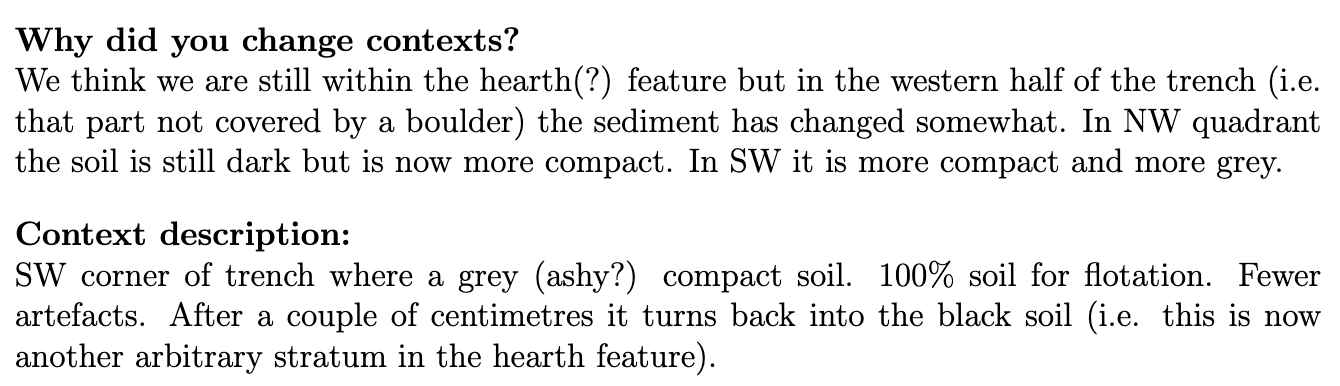
\includegraphics[keepaspectratio]{figures/context-description-transcribed.png}}
\caption{Transcribed section of a recording sheet describing the context
addressed in the observed
episode.}\label{fig-context-description-transcribed}
\end{figure}

\begin{figure}
\centering
\pandocbounded{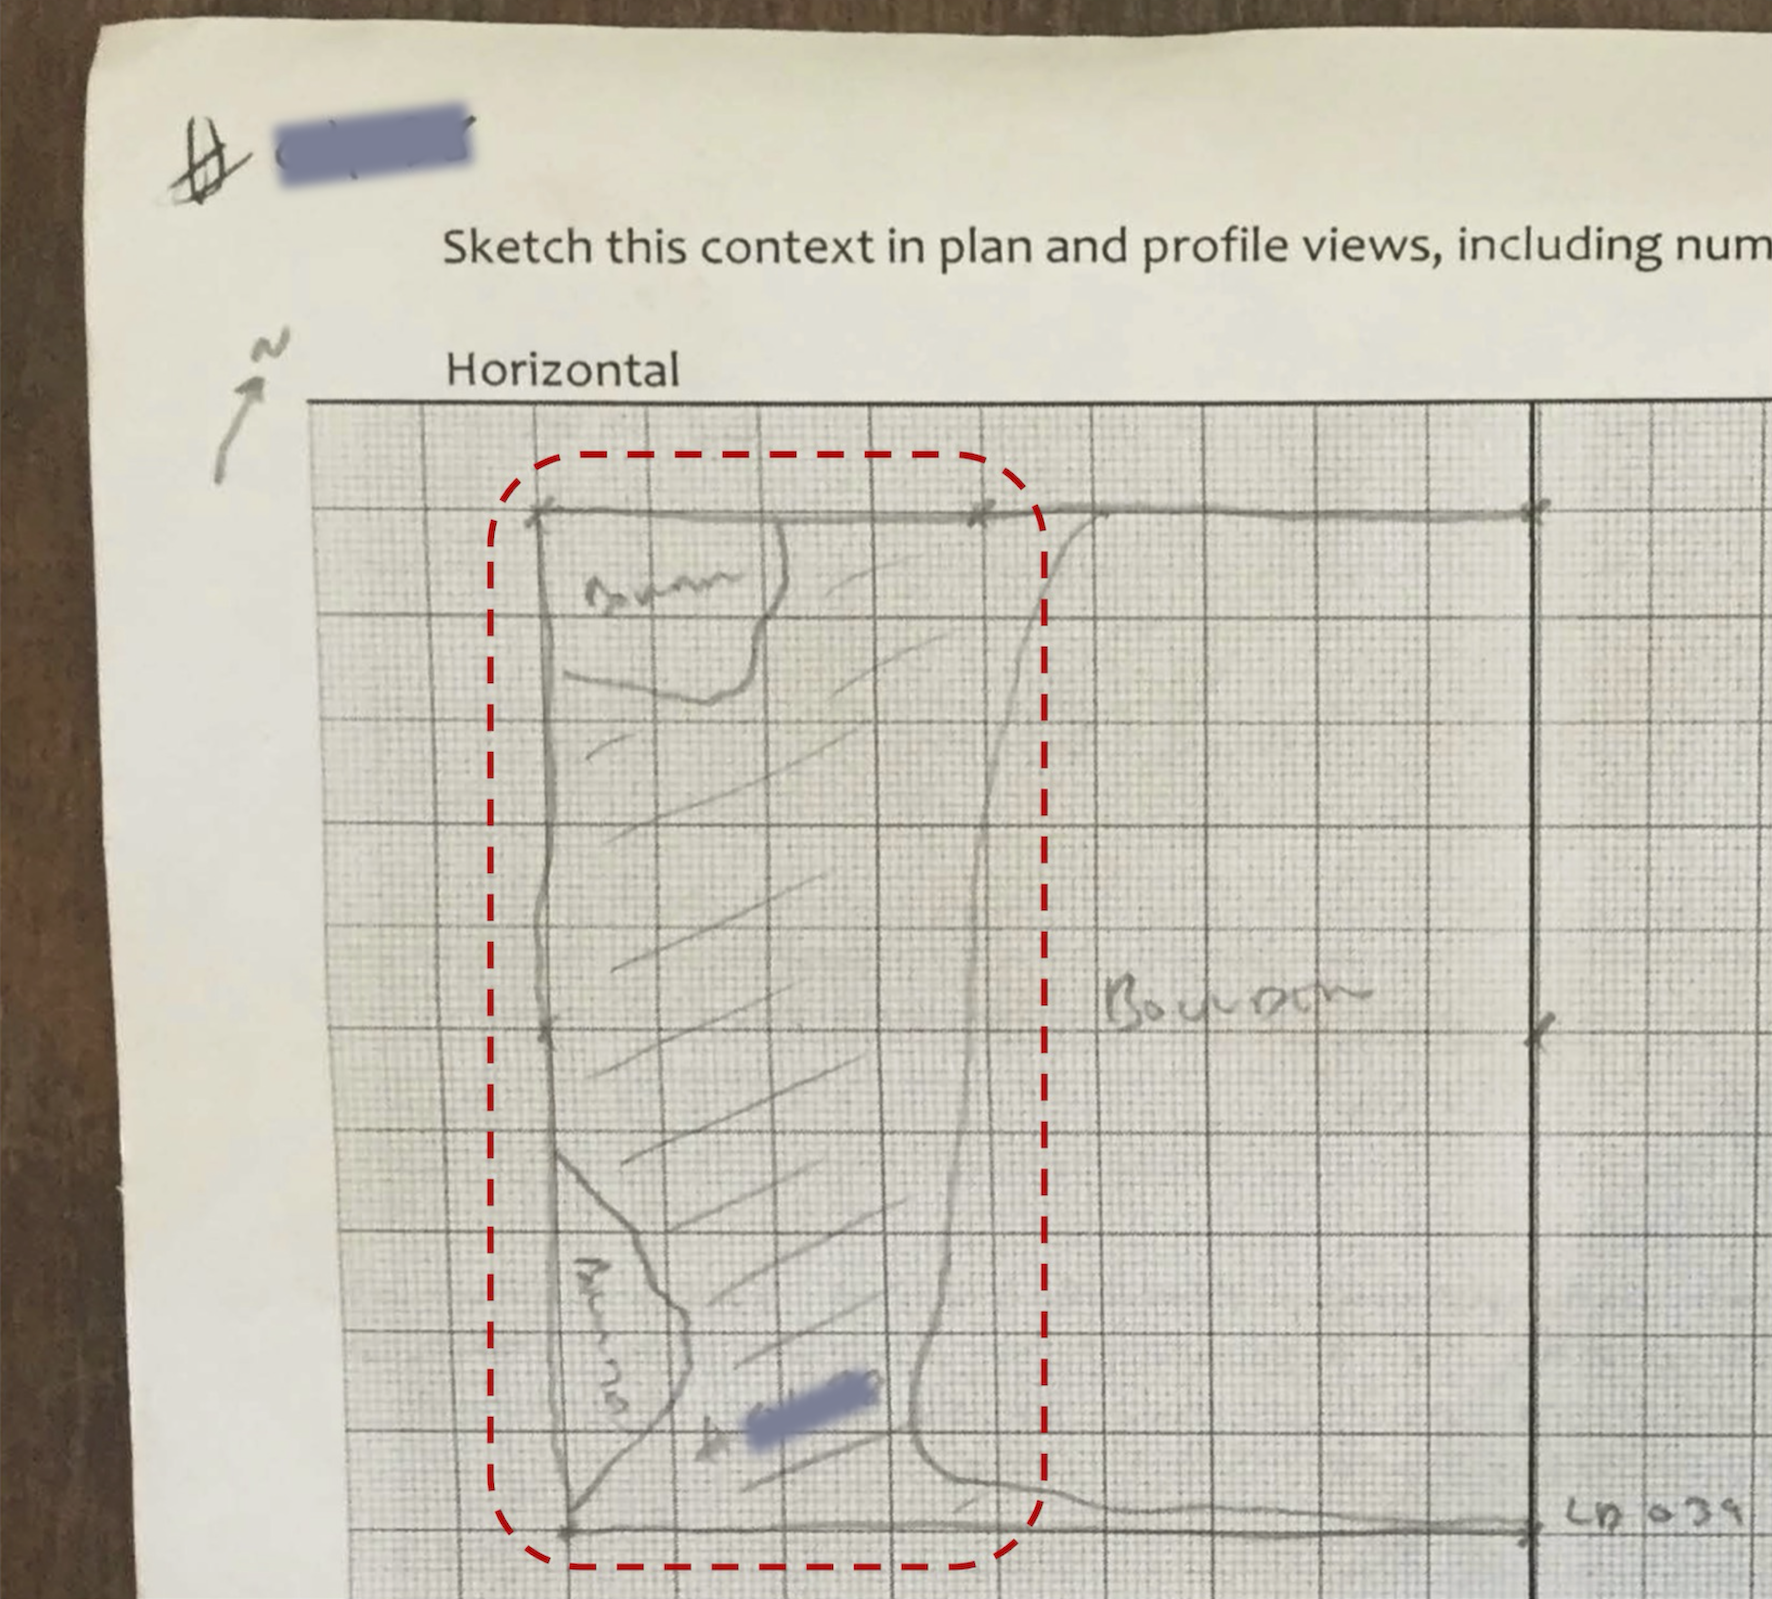
\includegraphics[keepaspectratio]{figures/context-sketch.png}}
\caption{Sketch of the base of a trench, portraying the context
addressed in the observed episode, boxed in
red.}\label{fig-context-sketch}
\end{figure}

\begin{figure}
\centering
\pandocbounded{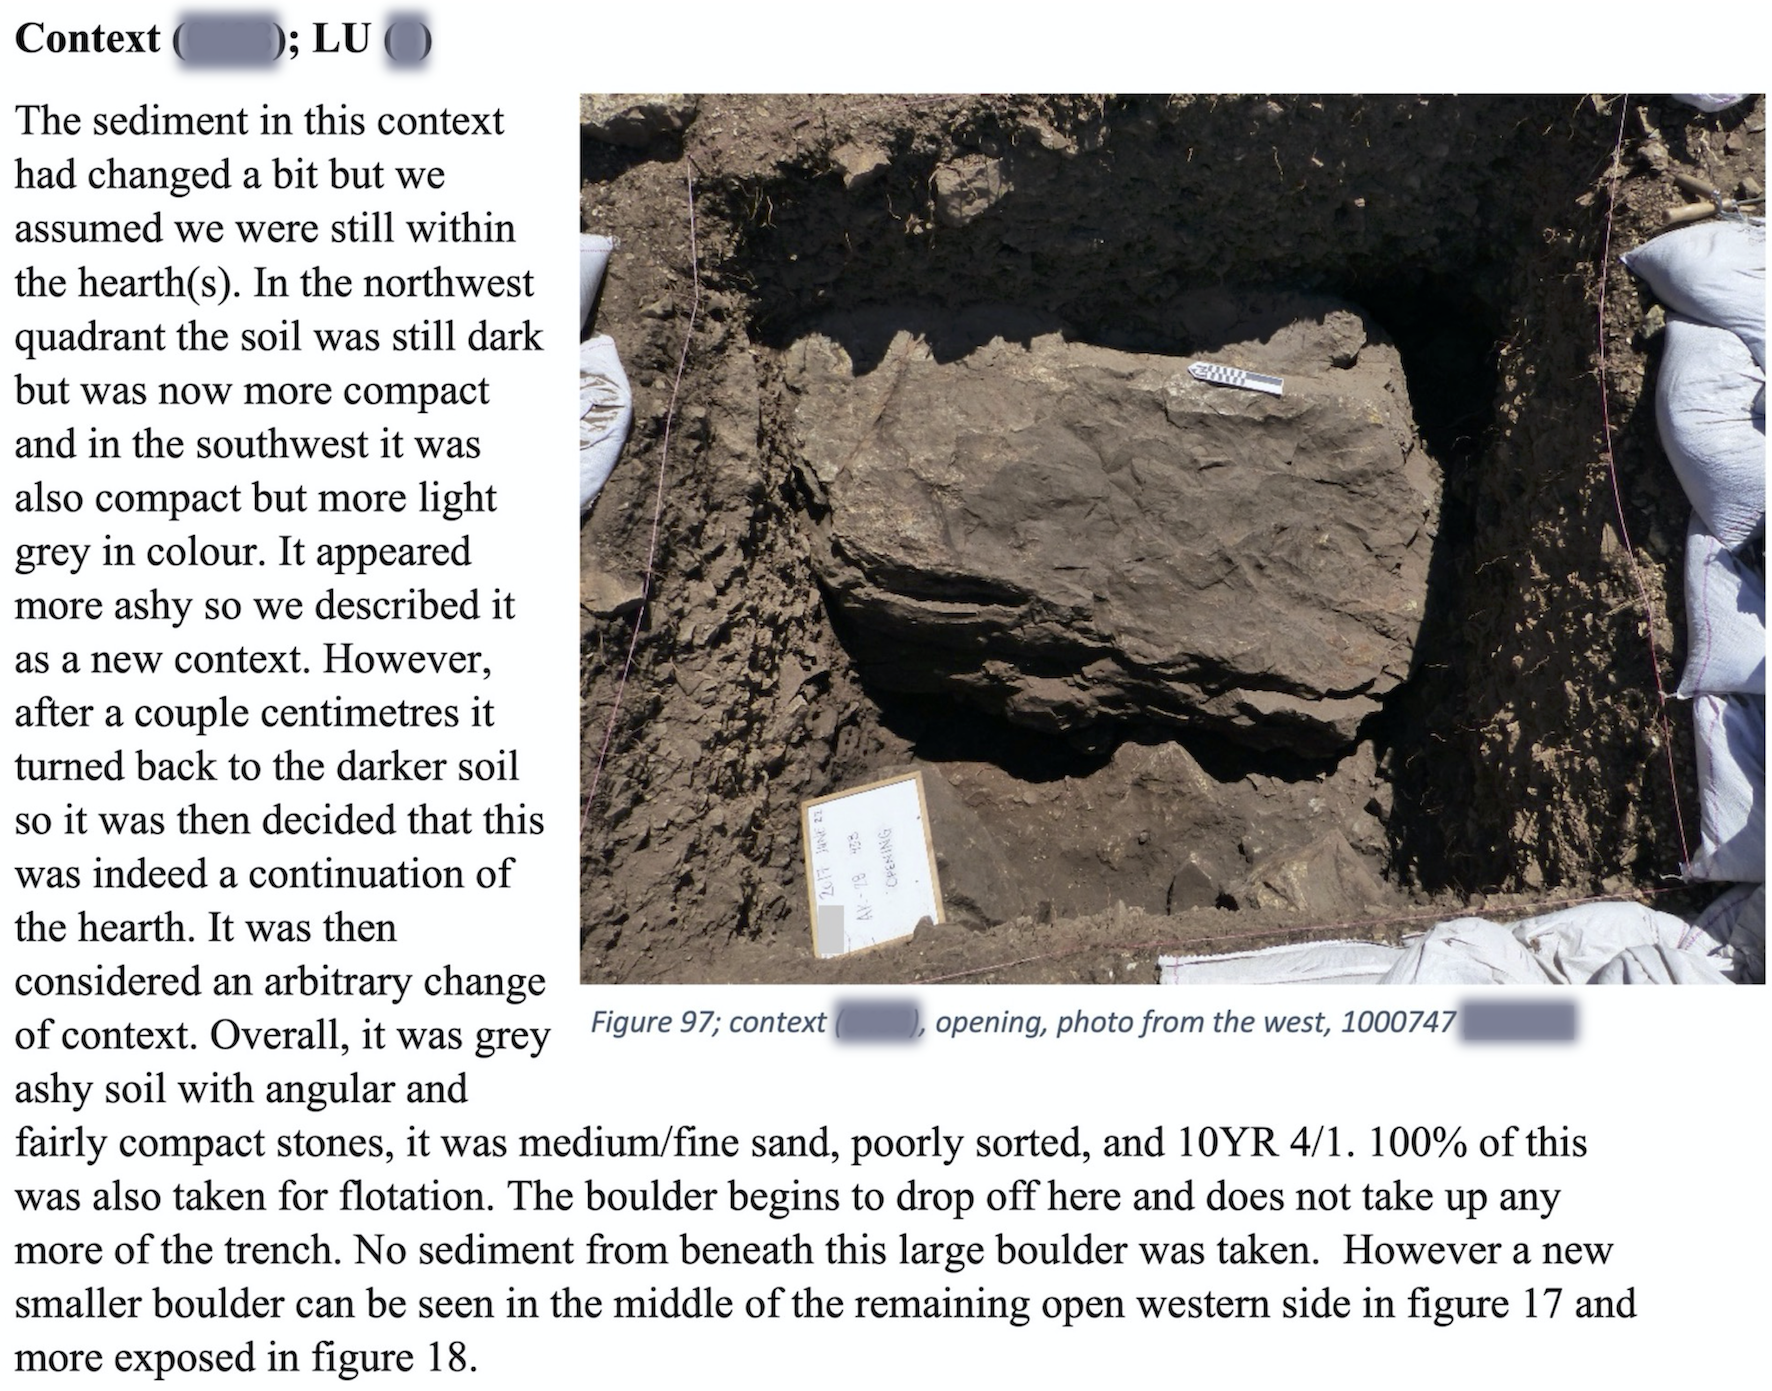
\includegraphics[keepaspectratio]{figures/context-report.png}}
\caption{Section of a trench report describing the context addressed in
the observed episode, and situating it as part of a lithostratigraphic
unit.}\label{fig-context-report}
\end{figure}

In particular, the tentativity and ambiguity that Jane and Basil
experienced while excavating this trench was one of its notable
properties, as elicited in the final trench report (see
\textcite{fig-context-report}). Additionally, the report described how
the contexts were eventually lumped together into a more concretely
defined ``lithostratigraphic unit,'' which was formally delimited using
nominal and standardized terminology. In this way, the report switched
back and forth between ambiguous and concrete representations, which
conveyed experiential and distant perspectives, respectively. This
resembles the tone switching that occurred in the conversation between
Jane and Basil, whereby Basil, as supervisor responsible for creating
formal documentation, re-presented Jane's experiences using more formal
terms. As such, this reflects an implicit recognition that there is
immense value in being able to share more nuanced perspectives on the
things that make up the archaeological record. At the same time, and in
contrast with truly situated records like those maintained in field
journals \autocite[cf.][]{batist2024a}, since the language documenting
such tentativity in the report remained largely impersonal and
observations were de-situated and disembodied.

It is notable that situated experiences were recorded in the
report-writing phase, and only by those acting in authoritative roles.
This parallels how field journals --- which are also records of situated
experiences --- are exclusively maintained by supervising personnel
\autocite{batist2024a}. These observations reflect the different kinds
of agency held by different actors in the project. Fieldworkers were
encouraged to shape their behaviour so that the information they
obtained was born as formal entities from the start, whereas those
responsible for presenting the record as part of a broader scope of work
were responsible for re-situating the data as products of
data-collection processes that they designed and dictated. Recognizing
the situatedness of data while they were being collected would have
warranted recognition of their limitations, which fieldworkers believed
would enable undisciplined data collection
behaviour.\textsuperscript{\hyperref[sec-A20]{A20}}

In other words, the constitution of archaeological records involved
temporarily suspending disbelief regarding the stability of
archaeological observations among fieldworkers, and then re-integration
of storied accounts about the record's origins by supervisors who were
granted greater creative agency. However, this was conditioned through
the use of language that rendered prior work as generic and non-situated
processes, thereby obscuring the agency of those whose work the report
was based on. Although not specifically targeted for this study, similar
tendencies may also be casually observed while recontextualizing prior
work as part of broader narratives at various scales --- in summaries
about a trench, an area, a site, and even an entire region.

\printbibliography

\end{document}
